\documentclass{article}
\usepackage[T1]{fontenc}
\usepackage{lmodern}
\usepackage{graphicx}
\usepackage{amsmath,amssymb}
\usepackage[a4paper,margin=2cm]{geometry}
\usepackage[absolute,overlay]{textpos}
\setlength{\TPHorizModule}{1mm}
\setlength{\TPVertModule}{1mm}
\usepackage[indonesian]{babel}
\usepackage{hyperref}
\setlength{\emergencystretch}{2em}
% unit: Halaman 58

\begin{document}

% === Halaman 58 (llm) ===

\begin{itemize}
    \item Kelompokkan "pesan" setiap berjarak 5, dimulai dari huruf cipherteks pertama, kedua, dan seterusnya. Setiap huruf pada posisi berjarak 5 pasti dienkripsi dengan huruf kunci yang sama.
\end{itemize}

\vspace{10mm}

\begin{tabular}{l l} 
Kelompok & Pesan \\
\hline
1 & LSLLMFLYJLVLLLYKWV \\
2 & JTQJPAJYQJTJKJJREH \\
3 & VNMVKVVVVLVRVEVFFZ \\
4 & BEEMAADNNHNCTHSTUN \\
5 & QZDAUTAFPKFMAUFTXP \\
\end{tabular}

\vspace{5mm}

\begin{tabular}{l} 
Huruf paling sering muncul \\
\hline
L \\
J \\
V \\
N \\
A \\
\end{tabular}

% deskripsi: Contoh pengelompokan cipherteks dengan huruf berwarna untuk menunjukkan pola pengulangan setiap 5 karakter.
% bbox normalisasi: [0.0500, 0.2900, 0.9200, 0.4500]
\begin{textblock*}{182.70mm}(10.50mm,86.13mm)
\noindent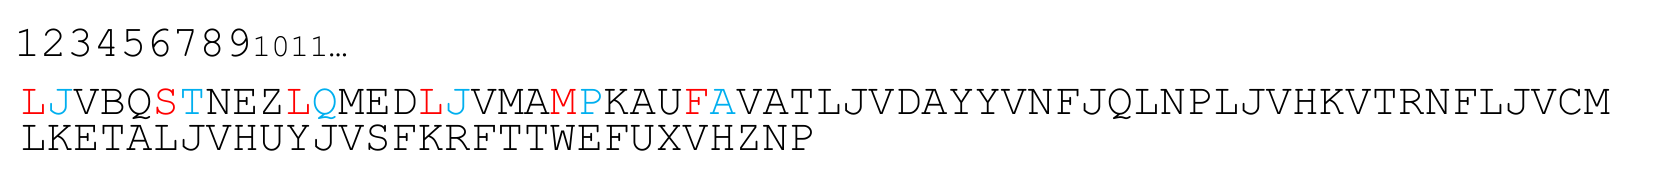
\includegraphics[width=182.70mm,height=47.52mm]{../../images/llm/page_058_img_01.png}%
\end{textblock*}

\end{document}
